\documentclass[a4paper,12pt]{article}
\usepackage{czech}
\usepackage[utf8]{inputenc}
\usepackage{a4wide}
\usepackage[dvipdfm]{graphicx}
\usepackage{graphics}
\usepackage{indentfirst}
\usepackage{fancyhdr}
\usepackage{setspace}
\usepackage{amsmath}
\usepackage{amssymb}
\usepackage{epsfig}

%%\usepackage{nopageno}
%%\usepackage{txfonts}
\usepackage[usenames]{color}
%\usepackage{multirow}

\begin{document}
\newcommand{\st}{^{\circ}}
\newcommand{\RJ}{\mbox{RJ}}
\newcommand{\mV}{\mbox{m}/\mbox{V}^2}

\section{Úkol}
\begin{enumerate}
    \item Vyneste do grafu disperzní relaci (spojitou závislost indexu lomu na vlnové délce) měřicího hranolu GoF3 pomocí údajů v tabulce 1.2.2.
    \item Stanovte disperzní relaci optických skel, jejich střední disperzi, relativní střední disperzi a Abbeovo číslo. Podle přiloženého výpisu z katalogu optických skel proveďte identifikaci měřených vzorků. Disperzní relaci vyneste do grafu.
    \item Stanovte teplotní závislost indexu lomu pro zadanou kapalinu pro tři různé vlnové délky v teplotním intervalu $20\st - 50\st$ . Zpracujte naměřené závislosti do grafu.
    \item Spočtěte chybu nepřímého měření indexů lomu pevných látek i kapalin a to obecně i numericky. V úkolu 2. spočtěte chybu nepřímého měření střední disperze, relativní střední disperze a Abbeova čísla. 
\end{enumerate}

\section{Teorie}
\subsection{Index lomu}
Index lomu charakterituje optické vlastnosti látky. Je definován vztahem
\begin{eqnarray}
N=\frac{c}{v},
\end{eqnarray}
kde $c$ je rychlost světla a $v$ rychlost, kterou se světlo šíří danou látkou.

Při měření například za pomoci Pulfrichovým refraktorem se dá pro pevné látky určit metodou mezního úhlu. 
Vzorec pro výpočet indexu lomu je dle \cite{text}
\begin{eqnarray}
N=\sqrt{N_1^2-\cos^2\gamma},
\label{N1}
\end{eqnarray}
kde $N_1$ je index lomu použitého hranolu a $\gamma$ měřený úhel.

Pro kapaliny se používá metoda vychylovací, pro který platí vztah
\begin{eqnarray}
N=\sqrt{N_1^2-\cos\gamma\sqrt{N_1^2-\cos^2\gamma}}
\label{N2}
\end{eqnarray}

\subsection{Abbeovo číslo}
Abbeovo číslo je definováno
\begin{eqnarray}
V=\frac{n_D-1}{n_F-n_C},
\end{eqnarray}
kde $n_D$ je index lomu pro vlnovou délku 589.2 nm, $n_F$ pro 486.1 nm a $n_C$ pro 656.3 .

\section{Měření}
\subsection{Disperzní relace hranolu GoF3}
Dle tabluky pro hranol GoF3 jsem vytvořil disperzní relace, která je na obrázku \ref{GGoF3}. Pro potřebu jiných spektrálních čar jsem této závislosti dofitoval 
křivku, která má předpis
\begin{eqnarray}
N=(1.7335\pm 0.0032)-(73.0\pm 6.6)\frac{1}{x}+(79200\pm 5100)\frac{1}{x^2}-(2.80\pm0.17)10^7\frac{1}{x^3}+(4.71\pm0.21)10^9\frac{1}{x^4}
\end{eqnarray}

\begin{figure}
% GNUPLOT: LaTeX picture with Postscript
\begingroup
  \makeatletter
  \providecommand\color[2][]{%
    \GenericError{(gnuplot) \space\space\space\@spaces}{%
      Package color not loaded in conjunction with
      terminal option `colourtext'%
    }{See the gnuplot documentation for explanation.%
    }{Either use 'blacktext' in gnuplot or load the package
      color.sty in LaTeX.}%
    \renewcommand\color[2][]{}%
  }%
  \providecommand\includegraphics[2][]{%
    \GenericError{(gnuplot) \space\space\space\@spaces}{%
      Package graphicx or graphics not loaded%
    }{See the gnuplot documentation for explanation.%
    }{The gnuplot epslatex terminal needs graphicx.sty or graphics.sty.}%
    \renewcommand\includegraphics[2][]{}%
  }%
  \providecommand\rotatebox[2]{#2}%
  \@ifundefined{ifGPcolor}{%
    \newif\ifGPcolor
    \GPcolorfalse
  }{}%
  \@ifundefined{ifGPblacktext}{%
    \newif\ifGPblacktext
    \GPblacktexttrue
  }{}%
  % define a \g@addto@macro without @ in the name:
  \let\gplgaddtomacro\g@addto@macro
  % define empty templates for all commands taking text:
  \gdef\gplbacktext{}%
  \gdef\gplfronttext{}%
  \makeatother
  \ifGPblacktext
    % no textcolor at all
    \def\colorrgb#1{}%
    \def\colorgray#1{}%
  \else
    % gray or color?
    \ifGPcolor
      \def\colorrgb#1{\color[rgb]{#1}}%
      \def\colorgray#1{\color[gray]{#1}}%
      \expandafter\def\csname LTw\endcsname{\color{white}}%
      \expandafter\def\csname LTb\endcsname{\color{black}}%
      \expandafter\def\csname LTa\endcsname{\color{black}}%
      \expandafter\def\csname LT0\endcsname{\color[rgb]{1,0,0}}%
      \expandafter\def\csname LT1\endcsname{\color[rgb]{0,1,0}}%
      \expandafter\def\csname LT2\endcsname{\color[rgb]{0,0,1}}%
      \expandafter\def\csname LT3\endcsname{\color[rgb]{1,0,1}}%
      \expandafter\def\csname LT4\endcsname{\color[rgb]{0,1,1}}%
      \expandafter\def\csname LT5\endcsname{\color[rgb]{1,1,0}}%
      \expandafter\def\csname LT6\endcsname{\color[rgb]{0,0,0}}%
      \expandafter\def\csname LT7\endcsname{\color[rgb]{1,0.3,0}}%
      \expandafter\def\csname LT8\endcsname{\color[rgb]{0.5,0.5,0.5}}%
    \else
      % gray
      \def\colorrgb#1{\color{black}}%
      \def\colorgray#1{\color[gray]{#1}}%
      \expandafter\def\csname LTw\endcsname{\color{white}}%
      \expandafter\def\csname LTb\endcsname{\color{black}}%
      \expandafter\def\csname LTa\endcsname{\color{black}}%
      \expandafter\def\csname LT0\endcsname{\color{black}}%
      \expandafter\def\csname LT1\endcsname{\color{black}}%
      \expandafter\def\csname LT2\endcsname{\color{black}}%
      \expandafter\def\csname LT3\endcsname{\color{black}}%
      \expandafter\def\csname LT4\endcsname{\color{black}}%
      \expandafter\def\csname LT5\endcsname{\color{black}}%
      \expandafter\def\csname LT6\endcsname{\color{black}}%
      \expandafter\def\csname LT7\endcsname{\color{black}}%
      \expandafter\def\csname LT8\endcsname{\color{black}}%
    \fi
  \fi
  \setlength{\unitlength}{0.0500bp}%
  \begin{picture}(7200.00,5040.00)%
    \gplgaddtomacro\gplbacktext{%
      \csname LTb\endcsname%
      \put(1078,704){\makebox(0,0)[r]{\strut{} 1.73}}%
      \put(1078,1286){\makebox(0,0)[r]{\strut{} 1.74}}%
      \put(1078,1867){\makebox(0,0)[r]{\strut{} 1.75}}%
      \put(1078,2449){\makebox(0,0)[r]{\strut{} 1.76}}%
      \put(1078,3030){\makebox(0,0)[r]{\strut{} 1.77}}%
      \put(1078,3612){\makebox(0,0)[r]{\strut{} 1.78}}%
      \put(1078,4193){\makebox(0,0)[r]{\strut{} 1.79}}%
      \put(1078,4775){\makebox(0,0)[r]{\strut{} 1.8}}%
      \put(1210,484){\makebox(0,0){\strut{} 400}}%
      \put(2142,484){\makebox(0,0){\strut{} 450}}%
      \put(3074,484){\makebox(0,0){\strut{} 500}}%
      \put(4007,484){\makebox(0,0){\strut{} 550}}%
      \put(4939,484){\makebox(0,0){\strut{} 600}}%
      \put(5871,484){\makebox(0,0){\strut{} 650}}%
      \put(6803,484){\makebox(0,0){\strut{} 700}}%
      \put(176,2739){\rotatebox{-270}{\makebox(0,0){\strut{}$N$}}}%
      \put(4006,154){\makebox(0,0){\strut{}$\lambda/\mbox{nm}$}}%
    }%
    \gplgaddtomacro\gplfronttext{%
      \csname LTb\endcsname%
      \put(5816,4602){\makebox(0,0)[r]{\strut{}tabelové hodnoty}}%
      \csname LTb\endcsname%
      \put(5816,4382){\makebox(0,0)[r]{\strut{}fitovaná záavislost}}%
    }%
    \gplbacktext
    \put(0,0){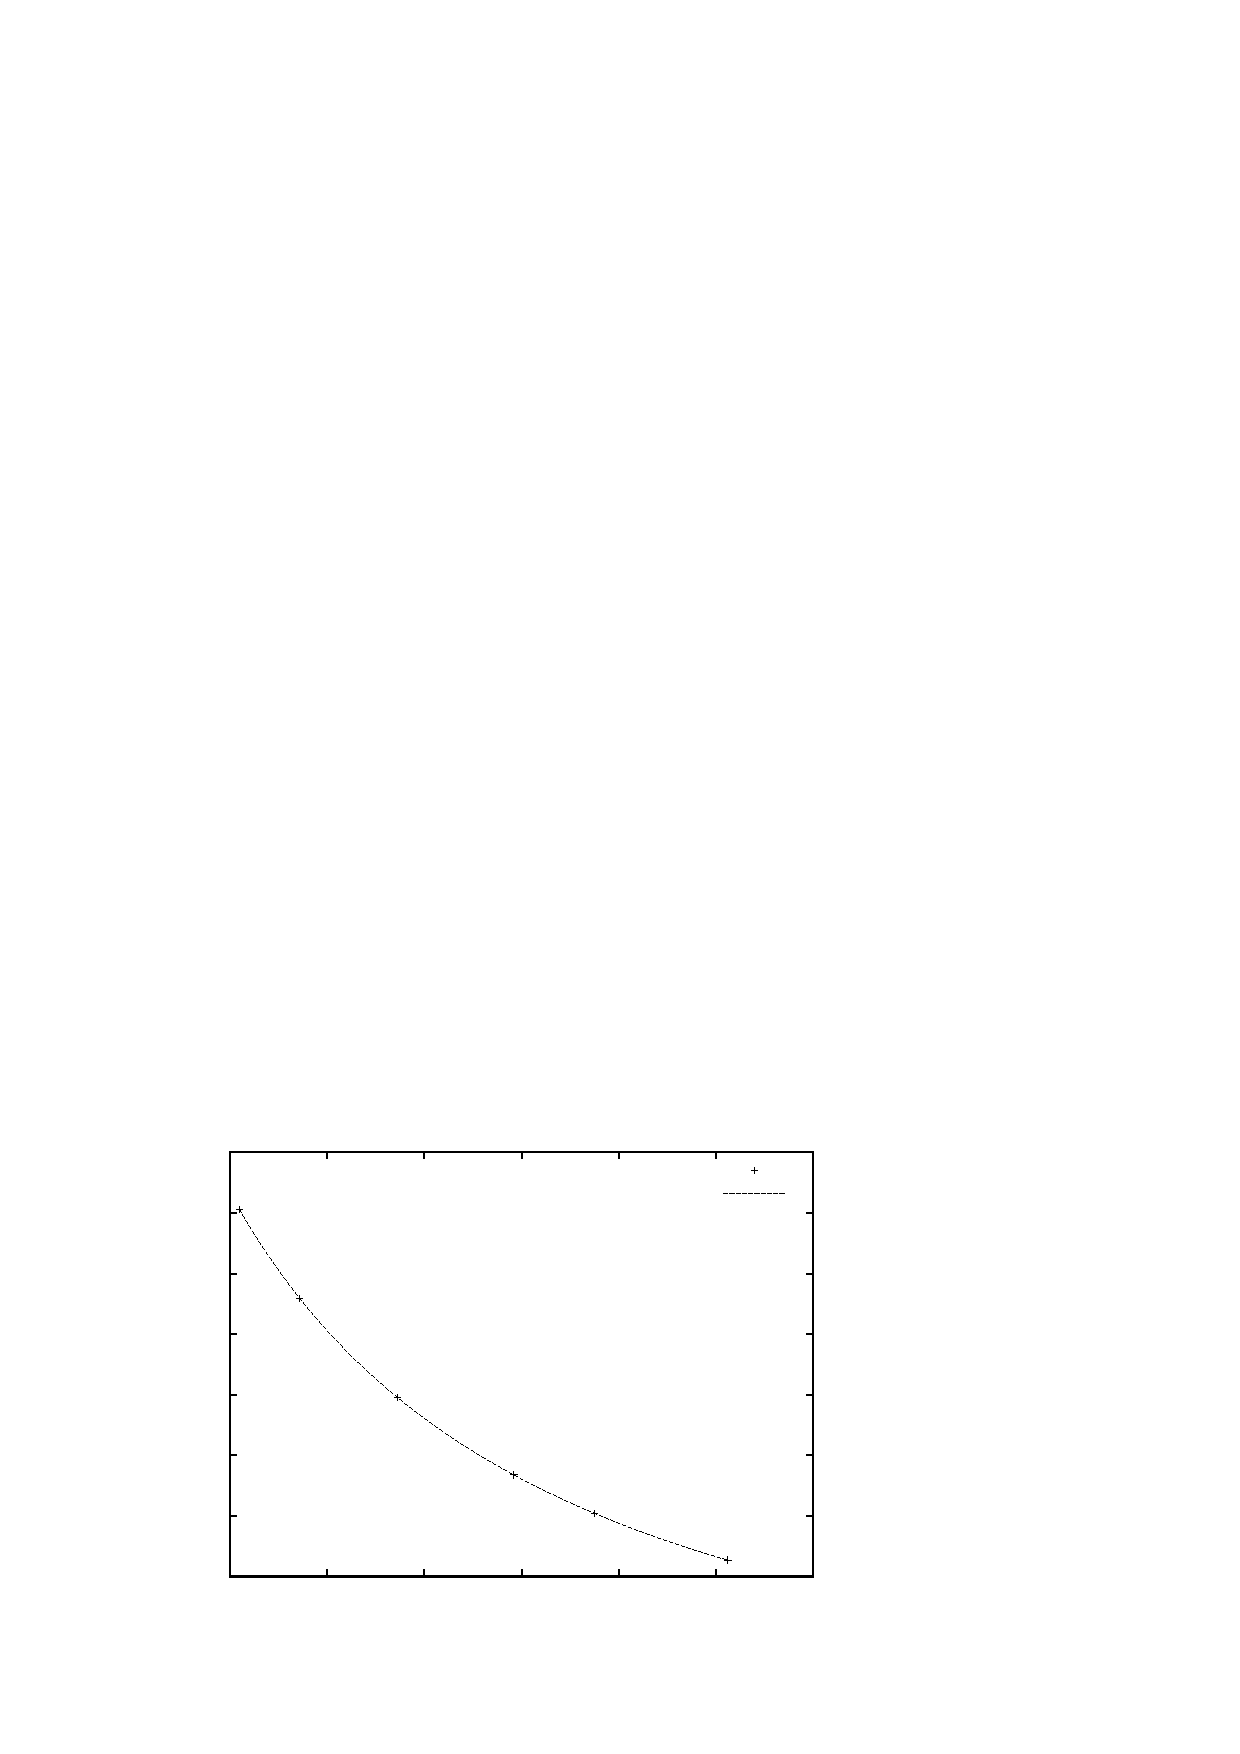
\includegraphics{GGoF3}}%
    \gplfronttext
  \end{picture}%
\endgroup

\caption{Disperzní relace hranolu GoF3}
\label{GGoF3}
\end{figure}



\subsection{Disperzní relace optických skel}
Vzorky 3 a 9 jsem umístil na měřící hranol a dle pokynů měřil mezní úhel pro jednotlivé čáry rtuťové výbojky a heliové trubice. Výsledky jsou v tabulkách 
\ref{T3}, \ref{T9} spolu s tabelovými hodnotami vlnových délek čar a dopočteným indexem lomu. Z výsledků jsem sestavil diperzní relaci pro oba vzorky, která je na obrázcích \ref{G3} a \ref{G9}. Nafitovaná křivka má předpis pro vzorek 9 předpis dle rovnice \ref{R9}. Pro vzorek 3 předpis kvůli velikosti chyby neuvádím.
\begin{eqnarray}
N_9=(4.254\pm 0.083)-(5500\pm 160)\frac{1}{x}+(4.25\pm 0.12)10^6\frac{1}{x^2}\\
-(1.45\pm0.04)10^9\frac{1}{x^3}+(1.85\pm0.05)10^11\frac{1}{x^4}
\label{R9}
\end{eqnarray}

\begin{table}
$$
\begin{array}{|c|c|c|c|}
\hline
\mbox{filtr}&   \varphi&    \lambda/\mbox{nm}&  N_2 \\ \hline
\mbox{e}&   49\st 55.95'&   546.1&  1.6248 \pm 0.0002 \\ \hline
\mbox{e}&   50\st 48.65'&   607.3&  1.6190 \pm 0.0002 \\ \hline
\mbox{g}&   47\st 22.9'&    435.8&  1.6418 \pm 0.0002 \\ \hline
\mbox{g}&   48\st 57.0'&    491.6&  1.6309 \pm 0.0002 \\ \hline
\mbox{d}& 50\st 20.0'&    579.1&  1.6204 \pm 0.0002 \\ \hline
\mbox{d}&   50\st 27.35'&   587.6&  1.6198 \pm 0.0002 \\ \hline
\end{array}
$$
\caption{Tabulka pro měření vzorku 9}
\label{T9}
\end{table}

\begin{table}
$$
\begin{array}{|c|c|c|c|}
\hline
\mbox{filtr}&   \varphi&    \lambda/\mbox{nm}&  N_2 \\ \hline
\mbox{e}&   30\st 38.2'&   546.1&  1.5201 \pm 0.0002 \\ \hline
\mbox{e}&   32\st 23.3'&   607.3&  1.5190 \pm 0.0002 \\ \hline
\mbox{g}&   28\st 37.5'&    491.6&  1.5233 \pm 0.0002 \\ \hline
\mbox{g}&   25\st 13.5'&    435.8&  1.5282 \pm 0.0002 \\ \hline
\mbox{h}& 21\st 59.75'&    404.7&  1.5318 \pm 0.0002 \\ \hline
\mbox{F}&    31\st 25.6'&    577.0&  1.5186 \pm 0.0002 \\ \hline
\mbox{F}&   31\st 29.45'&   579.1&  1.5186 \pm 0.0002 \\ \hline
\mbox{h}&   31\st 41.85'&   587.6&  1.5183 \pm 0.0002 \\ \hline
\end{array}
$$
\caption{Tabulka pro měření vzorku 3}
\label{T3}
\end{table}

\begin{figure}
% GNUPLOT: LaTeX picture with Postscript
\begingroup
  \makeatletter
  \providecommand\color[2][]{%
    \GenericError{(gnuplot) \space\space\space\@spaces}{%
      Package color not loaded in conjunction with
      terminal option `colourtext'%
    }{See the gnuplot documentation for explanation.%
    }{Either use 'blacktext' in gnuplot or load the package
      color.sty in LaTeX.}%
    \renewcommand\color[2][]{}%
  }%
  \providecommand\includegraphics[2][]{%
    \GenericError{(gnuplot) \space\space\space\@spaces}{%
      Package graphicx or graphics not loaded%
    }{See the gnuplot documentation for explanation.%
    }{The gnuplot epslatex terminal needs graphicx.sty or graphics.sty.}%
    \renewcommand\includegraphics[2][]{}%
  }%
  \providecommand\rotatebox[2]{#2}%
  \@ifundefined{ifGPcolor}{%
    \newif\ifGPcolor
    \GPcolorfalse
  }{}%
  \@ifundefined{ifGPblacktext}{%
    \newif\ifGPblacktext
    \GPblacktexttrue
  }{}%
  % define a \g@addto@macro without @ in the name:
  \let\gplgaddtomacro\g@addto@macro
  % define empty templates for all commands taking text:
  \gdef\gplbacktext{}%
  \gdef\gplfronttext{}%
  \makeatother
  \ifGPblacktext
    % no textcolor at all
    \def\colorrgb#1{}%
    \def\colorgray#1{}%
  \else
    % gray or color?
    \ifGPcolor
      \def\colorrgb#1{\color[rgb]{#1}}%
      \def\colorgray#1{\color[gray]{#1}}%
      \expandafter\def\csname LTw\endcsname{\color{white}}%
      \expandafter\def\csname LTb\endcsname{\color{black}}%
      \expandafter\def\csname LTa\endcsname{\color{black}}%
      \expandafter\def\csname LT0\endcsname{\color[rgb]{1,0,0}}%
      \expandafter\def\csname LT1\endcsname{\color[rgb]{0,1,0}}%
      \expandafter\def\csname LT2\endcsname{\color[rgb]{0,0,1}}%
      \expandafter\def\csname LT3\endcsname{\color[rgb]{1,0,1}}%
      \expandafter\def\csname LT4\endcsname{\color[rgb]{0,1,1}}%
      \expandafter\def\csname LT5\endcsname{\color[rgb]{1,1,0}}%
      \expandafter\def\csname LT6\endcsname{\color[rgb]{0,0,0}}%
      \expandafter\def\csname LT7\endcsname{\color[rgb]{1,0.3,0}}%
      \expandafter\def\csname LT8\endcsname{\color[rgb]{0.5,0.5,0.5}}%
    \else
      % gray
      \def\colorrgb#1{\color{black}}%
      \def\colorgray#1{\color[gray]{#1}}%
      \expandafter\def\csname LTw\endcsname{\color{white}}%
      \expandafter\def\csname LTb\endcsname{\color{black}}%
      \expandafter\def\csname LTa\endcsname{\color{black}}%
      \expandafter\def\csname LT0\endcsname{\color{black}}%
      \expandafter\def\csname LT1\endcsname{\color{black}}%
      \expandafter\def\csname LT2\endcsname{\color{black}}%
      \expandafter\def\csname LT3\endcsname{\color{black}}%
      \expandafter\def\csname LT4\endcsname{\color{black}}%
      \expandafter\def\csname LT5\endcsname{\color{black}}%
      \expandafter\def\csname LT6\endcsname{\color{black}}%
      \expandafter\def\csname LT7\endcsname{\color{black}}%
      \expandafter\def\csname LT8\endcsname{\color{black}}%
    \fi
  \fi
  \setlength{\unitlength}{0.0500bp}%
  \begin{picture}(7200.00,5040.00)%
    \gplgaddtomacro\gplbacktext{%
      \csname LTb\endcsname%
      \put(1210,704){\makebox(0,0)[r]{\strut{} 1.518}}%
      \put(1210,1286){\makebox(0,0)[r]{\strut{} 1.52}}%
      \put(1210,1867){\makebox(0,0)[r]{\strut{} 1.522}}%
      \put(1210,2449){\makebox(0,0)[r]{\strut{} 1.524}}%
      \put(1210,3030){\makebox(0,0)[r]{\strut{} 1.526}}%
      \put(1210,3612){\makebox(0,0)[r]{\strut{} 1.528}}%
      \put(1210,4193){\makebox(0,0)[r]{\strut{} 1.53}}%
      \put(1210,4775){\makebox(0,0)[r]{\strut{} 1.532}}%
      \put(1342,484){\makebox(0,0){\strut{} 400}}%
      \put(2434,484){\makebox(0,0){\strut{} 450}}%
      \put(3526,484){\makebox(0,0){\strut{} 500}}%
      \put(4619,484){\makebox(0,0){\strut{} 550}}%
      \put(5711,484){\makebox(0,0){\strut{} 600}}%
      \put(6803,484){\makebox(0,0){\strut{} 650}}%
      \put(176,2739){\rotatebox{-270}{\makebox(0,0){\strut{}$N$}}}%
      \put(4072,154){\makebox(0,0){\strut{}$\lambda/\mbox{nm}$}}%
    }%
    \gplgaddtomacro\gplfronttext{%
      \csname LTb\endcsname%
      \put(5816,4602){\makebox(0,0)[r]{\strut{}naměřené hodnoty}}%
      \csname LTb\endcsname%
      \put(5816,4382){\makebox(0,0)[r]{\strut{}fitovaná záavislost}}%
    }%
    \gplbacktext
    \put(0,0){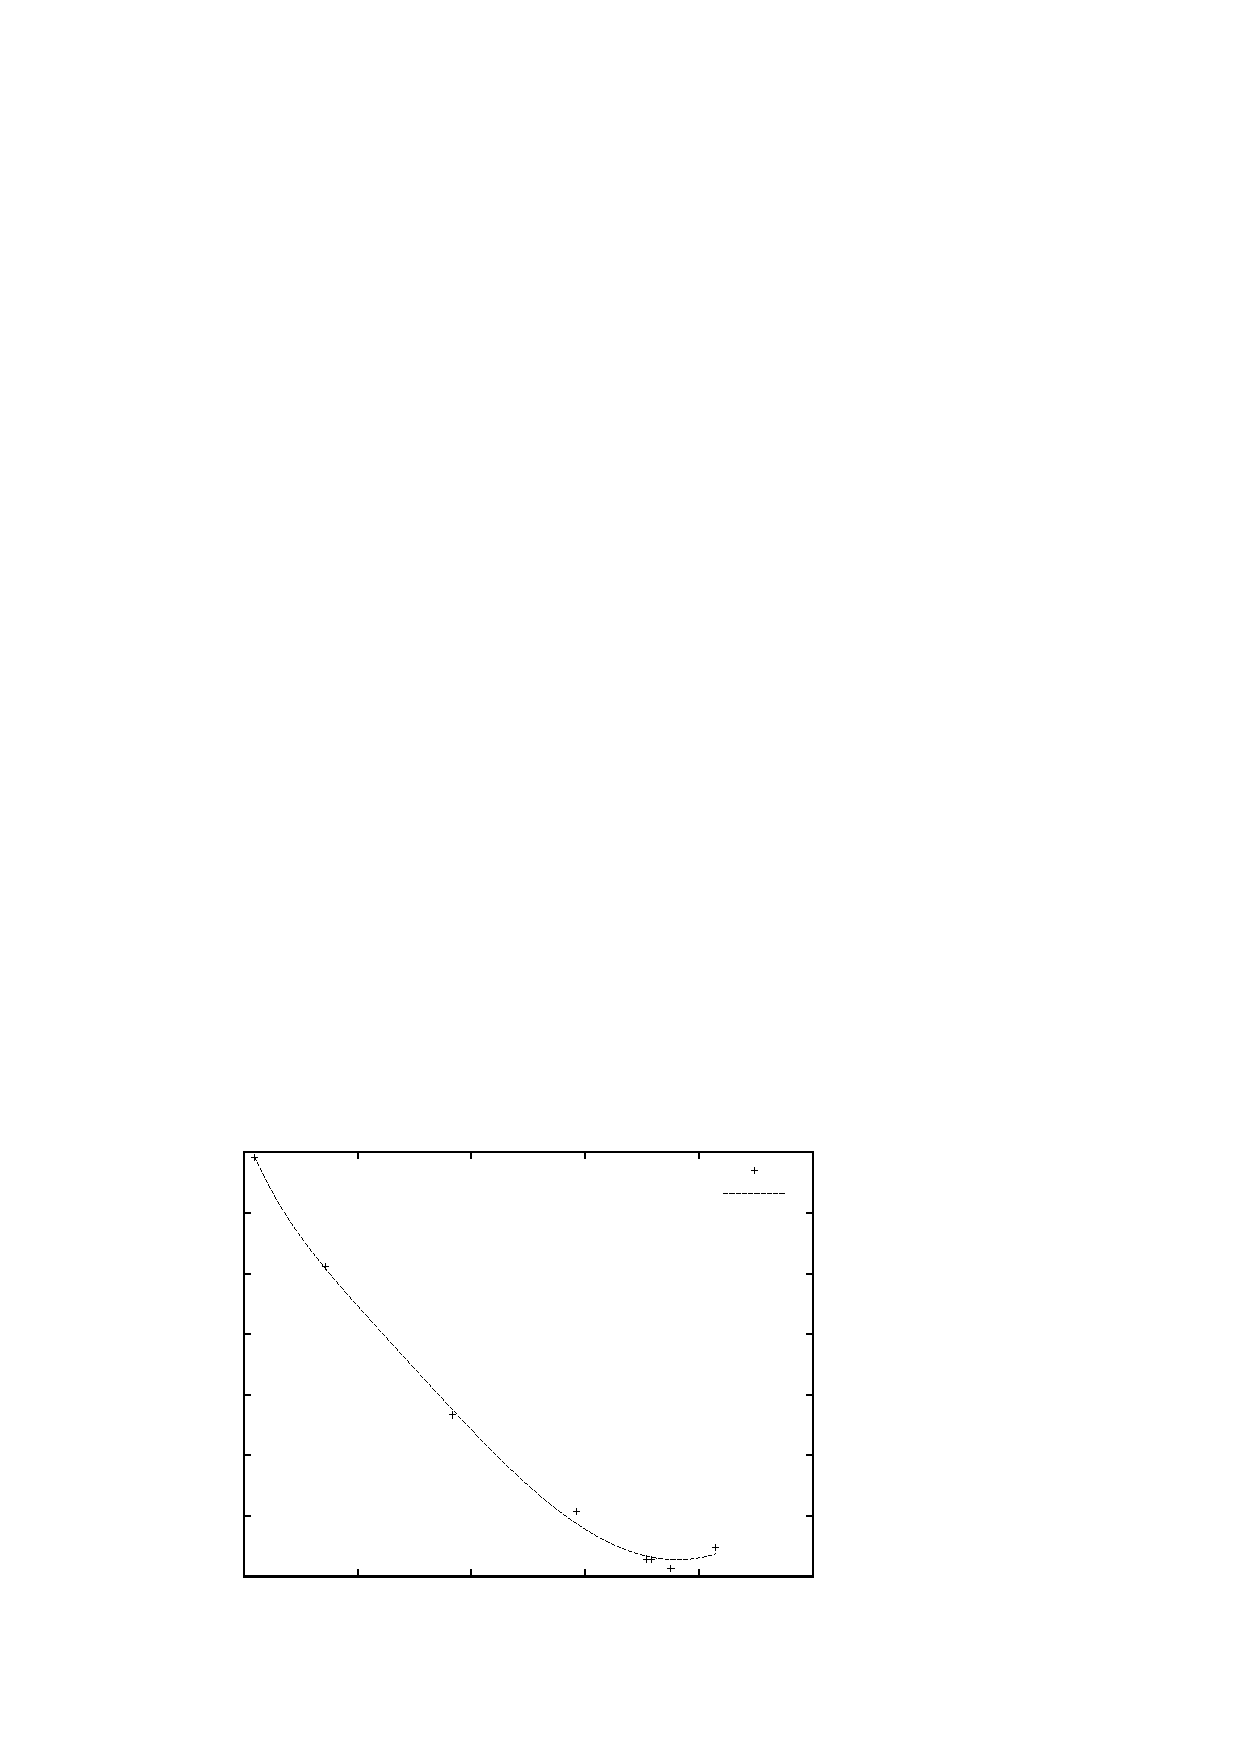
\includegraphics{G3}}%
    \gplfronttext
  \end{picture}%
\endgroup

\caption{Disperzní relace vzorku 3}
\label{G3}
\end{figure}

\begin{figure}
% GNUPLOT: LaTeX picture with Postscript
\begingroup
  \makeatletter
  \providecommand\color[2][]{%
    \GenericError{(gnuplot) \space\space\space\@spaces}{%
      Package color not loaded in conjunction with
      terminal option `colourtext'%
    }{See the gnuplot documentation for explanation.%
    }{Either use 'blacktext' in gnuplot or load the package
      color.sty in LaTeX.}%
    \renewcommand\color[2][]{}%
  }%
  \providecommand\includegraphics[2][]{%
    \GenericError{(gnuplot) \space\space\space\@spaces}{%
      Package graphicx or graphics not loaded%
    }{See the gnuplot documentation for explanation.%
    }{The gnuplot epslatex terminal needs graphicx.sty or graphics.sty.}%
    \renewcommand\includegraphics[2][]{}%
  }%
  \providecommand\rotatebox[2]{#2}%
  \@ifundefined{ifGPcolor}{%
    \newif\ifGPcolor
    \GPcolorfalse
  }{}%
  \@ifundefined{ifGPblacktext}{%
    \newif\ifGPblacktext
    \GPblacktexttrue
  }{}%
  % define a \g@addto@macro without @ in the name:
  \let\gplgaddtomacro\g@addto@macro
  % define empty templates for all commands taking text:
  \gdef\gplbacktext{}%
  \gdef\gplfronttext{}%
  \makeatother
  \ifGPblacktext
    % no textcolor at all
    \def\colorrgb#1{}%
    \def\colorgray#1{}%
  \else
    % gray or color?
    \ifGPcolor
      \def\colorrgb#1{\color[rgb]{#1}}%
      \def\colorgray#1{\color[gray]{#1}}%
      \expandafter\def\csname LTw\endcsname{\color{white}}%
      \expandafter\def\csname LTb\endcsname{\color{black}}%
      \expandafter\def\csname LTa\endcsname{\color{black}}%
      \expandafter\def\csname LT0\endcsname{\color[rgb]{1,0,0}}%
      \expandafter\def\csname LT1\endcsname{\color[rgb]{0,1,0}}%
      \expandafter\def\csname LT2\endcsname{\color[rgb]{0,0,1}}%
      \expandafter\def\csname LT3\endcsname{\color[rgb]{1,0,1}}%
      \expandafter\def\csname LT4\endcsname{\color[rgb]{0,1,1}}%
      \expandafter\def\csname LT5\endcsname{\color[rgb]{1,1,0}}%
      \expandafter\def\csname LT6\endcsname{\color[rgb]{0,0,0}}%
      \expandafter\def\csname LT7\endcsname{\color[rgb]{1,0.3,0}}%
      \expandafter\def\csname LT8\endcsname{\color[rgb]{0.5,0.5,0.5}}%
    \else
      % gray
      \def\colorrgb#1{\color{black}}%
      \def\colorgray#1{\color[gray]{#1}}%
      \expandafter\def\csname LTw\endcsname{\color{white}}%
      \expandafter\def\csname LTb\endcsname{\color{black}}%
      \expandafter\def\csname LTa\endcsname{\color{black}}%
      \expandafter\def\csname LT0\endcsname{\color{black}}%
      \expandafter\def\csname LT1\endcsname{\color{black}}%
      \expandafter\def\csname LT2\endcsname{\color{black}}%
      \expandafter\def\csname LT3\endcsname{\color{black}}%
      \expandafter\def\csname LT4\endcsname{\color{black}}%
      \expandafter\def\csname LT5\endcsname{\color{black}}%
      \expandafter\def\csname LT6\endcsname{\color{black}}%
      \expandafter\def\csname LT7\endcsname{\color{black}}%
      \expandafter\def\csname LT8\endcsname{\color{black}}%
    \fi
  \fi
  \setlength{\unitlength}{0.0500bp}%
  \begin{picture}(7200.00,5040.00)%
    \gplgaddtomacro\gplbacktext{%
      \csname LTb\endcsname%
      \put(1210,704){\makebox(0,0)[r]{\strut{} 1.615}}%
      \put(1210,1382){\makebox(0,0)[r]{\strut{} 1.62}}%
      \put(1210,2061){\makebox(0,0)[r]{\strut{} 1.625}}%
      \put(1210,2739){\makebox(0,0)[r]{\strut{} 1.63}}%
      \put(1210,3418){\makebox(0,0)[r]{\strut{} 1.635}}%
      \put(1210,4096){\makebox(0,0)[r]{\strut{} 1.64}}%
      \put(1210,4775){\makebox(0,0)[r]{\strut{} 1.645}}%
      \put(1342,484){\makebox(0,0){\strut{} 420}}%
      \put(1888,484){\makebox(0,0){\strut{} 440}}%
      \put(2434,484){\makebox(0,0){\strut{} 460}}%
      \put(2980,484){\makebox(0,0){\strut{} 480}}%
      \put(3526,484){\makebox(0,0){\strut{} 500}}%
      \put(4072,484){\makebox(0,0){\strut{} 520}}%
      \put(4619,484){\makebox(0,0){\strut{} 540}}%
      \put(5165,484){\makebox(0,0){\strut{} 560}}%
      \put(5711,484){\makebox(0,0){\strut{} 580}}%
      \put(6257,484){\makebox(0,0){\strut{} 600}}%
      \put(6803,484){\makebox(0,0){\strut{} 620}}%
      \put(176,2739){\rotatebox{-270}{\makebox(0,0){\strut{}$N$}}}%
      \put(4072,154){\makebox(0,0){\strut{}$\lambda/\mbox{nm}$}}%
    }%
    \gplgaddtomacro\gplfronttext{%
      \csname LTb\endcsname%
      \put(5816,4602){\makebox(0,0)[r]{\strut{}naměřené hodnoty}}%
      \csname LTb\endcsname%
      \put(5816,4382){\makebox(0,0)[r]{\strut{}fitovaná záavislost}}%
    }%
    \gplbacktext
    \put(0,0){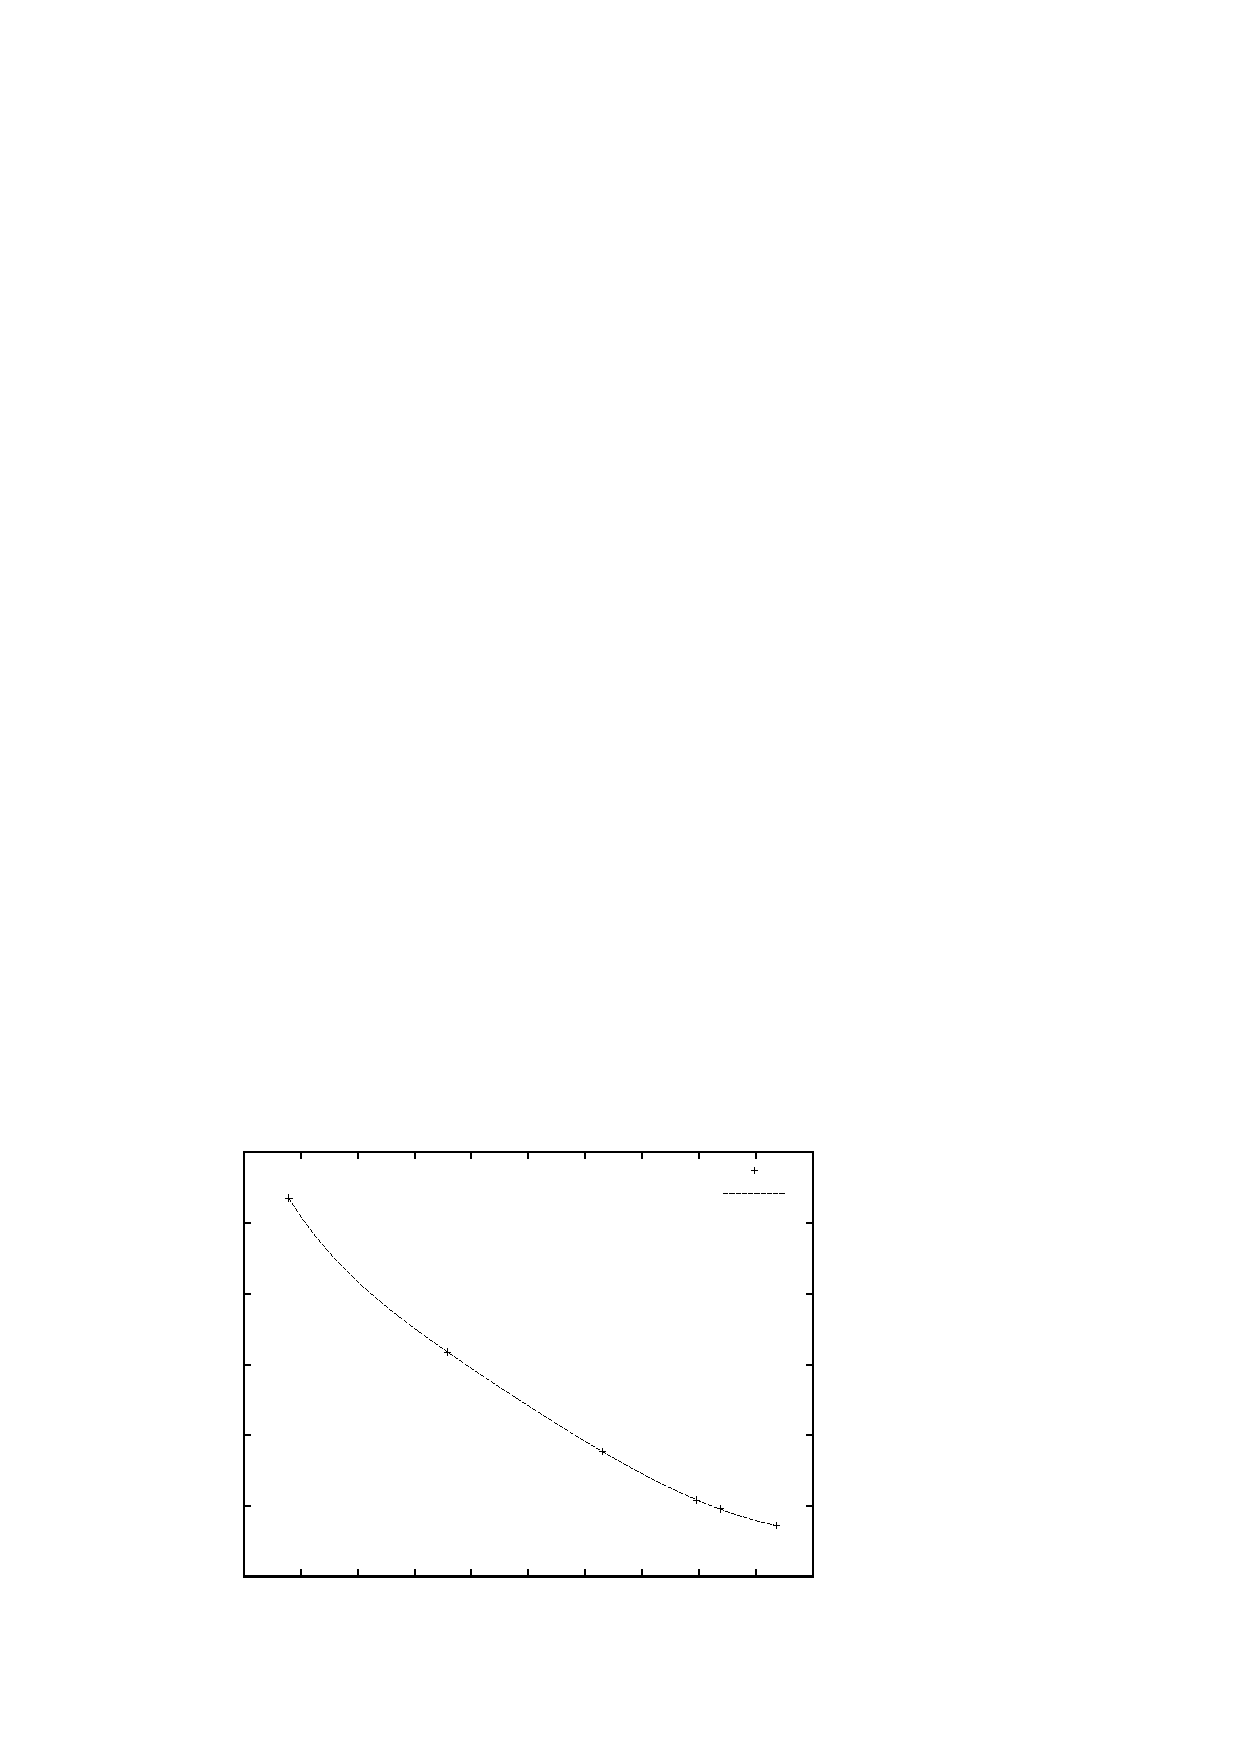
\includegraphics{G9}}%
    \gplfronttext
  \end{picture}%
\endgroup

\caption{Disperzní relace vzorku 9}
\label{G9}
\end{figure}


Střední disperze a relativní disperze obou vzorků jsou v tabulce \ref{TDis}. Chyby těchto hodnot jsou 0.2 \% pro střední disperzi a 0.4 \% pro relativní disperzi.

\begin{table}
$$
\begin{array}{|c|c|c|}
\hline
&   9&  3 \\ \hline
\mbox{F-C}& 0.0128& 0.0050 \\ \hline
\mbox{F-d}& 0.0120& 0.0054 \\ \hline
\mbox{F-e}& 0.0078& 0.0038 \\ \hline
\mbox{g-F}& 0.0101& 0.0043 \\ \hline
\mbox{d-C}& 0.0008& -0.0004 \\ \hline
\mbox{F-d/F-C}& 0.936&  1.081 \\ \hline
\mbox{F-e/F-C}& 0.609&  0.761 \\ \hline
\mbox{g-F/F-C}& 0.787&  0.855 \\ \hline
\mbox{d-C/F-C}& 0.064&  -0.080 \\ \hline
\end{array}
$$
\caption{Střední a relativní disperze vzorků}
\label{TDis}
\end{table}





Význačné hodnoty indexu lomu vzorlů jsou pro srovnání s tabulkou
\begin{eqnarray}
N_{d3}=(1.5185 \pm 0.0002)\mbox{nm} \\
N_{d9}=(1.6198 \pm 0.0002)\mbox{nm}
\end{eqnarray}
a Abbeovo čislo
\begin{eqnarray}
V_3=103.0 \\
V_9=48.27
\end{eqnarray}

Ve srovnání s tabulkou laboratorních skel se vzorek 3 jeví jako sklo BK 7 a vzorek 9 jako sklo F2.



\subsection{Závislost indexu lomu na teplotě}
Mnou vybrané tři vlnové délky pro pozorování teplotní závislosti indexu lomu byly 404.7 nm, 546.1 nm a 579.1 nm. Hodnoty jsem odečital přibližně po $3\st$C. 
Výsledky celého měření jsou v tabulce \ref{TT} a na obrázku \ref{GT}.

Naměřené hodnoty odpovídají ethanolu, což potvrzuje i charakteristická vůně. (Jednalo se o vzorek 1)

\begin{table}
$$
\begin{array}{|c|c|c|c|c|c|c|}
\hline
\mbox{t}/\st\mbox{C}&   \varphi_1&  N_1&    \varphi_2&  N_2&    \varphi_3&  N_3 \\ \hline
22& 36\st 10.0'&    1.3843&  40\st 47.85'&   1.3641&  41\st 32.75'&   1.3618 \\ \hline
26& 36\st 4.0'& 1.3839& 40\st 45.0'&    1.3639&    41\st 30.5'&    1.3616 \\ \hline
29& 35\st 45.45'&   1.3825& 40\st 26.8'&    1.3623& 41\st 10.8'&    1.3600 \\ \hline
32& 35\st 28.7'&    1.3813& 40\st 14.9'&    1.3613& 41\st 1.5'& 1.3591 \\ \hline
35& 35\st 12.9'&    1.3802& 39\st 58.3'&    1.3600& 40\st 43.2'&    1.3576 \\ \hline
38& 34\st 46.4'&    1.3783& 39\st 39.1'&    1.3584& 40\st 26.85'&   1.3562 \\ \hline
41& 34\st 33.3'&    1.3774& 39\st 25.7'&    1.3573& 40\st 12.0'&    1.3550 \\ \hline
44& 34\st 17.6'&    1.3763& 39\st 15.05'&   1.3565& 40\st 3.45'&    1.3543 \\ \hline
47& 34\st 5.75'&    1.3755& 39\st 2.4'&     1.3554& 39\st 48.7'&    1.3531 \\ \hline
50& 33\st 46.35'&   1.3741& 38\st 49.95'&   1.3544& 39\st 38.8'&    1.3522 \\ \hline
\end{array}
$$
\caption{Hodnoty z měření indexu lomu kapaliny v závislosti na teplotě.}
\label{TT}
\end{table}

\begin{figure}
% GNUPLOT: LaTeX picture with Postscript
\begingroup
  \makeatletter
  \providecommand\color[2][]{%
    \GenericError{(gnuplot) \space\space\space\@spaces}{%
      Package color not loaded in conjunction with
      terminal option `colourtext'%
    }{See the gnuplot documentation for explanation.%
    }{Either use 'blacktext' in gnuplot or load the package
      color.sty in LaTeX.}%
    \renewcommand\color[2][]{}%
  }%
  \providecommand\includegraphics[2][]{%
    \GenericError{(gnuplot) \space\space\space\@spaces}{%
      Package graphicx or graphics not loaded%
    }{See the gnuplot documentation for explanation.%
    }{The gnuplot epslatex terminal needs graphicx.sty or graphics.sty.}%
    \renewcommand\includegraphics[2][]{}%
  }%
  \providecommand\rotatebox[2]{#2}%
  \@ifundefined{ifGPcolor}{%
    \newif\ifGPcolor
    \GPcolorfalse
  }{}%
  \@ifundefined{ifGPblacktext}{%
    \newif\ifGPblacktext
    \GPblacktexttrue
  }{}%
  % define a \g@addto@macro without @ in the name:
  \let\gplgaddtomacro\g@addto@macro
  % define empty templates for all commands taking text:
  \gdef\gplbacktext{}%
  \gdef\gplfronttext{}%
  \makeatother
  \ifGPblacktext
    % no textcolor at all
    \def\colorrgb#1{}%
    \def\colorgray#1{}%
  \else
    % gray or color?
    \ifGPcolor
      \def\colorrgb#1{\color[rgb]{#1}}%
      \def\colorgray#1{\color[gray]{#1}}%
      \expandafter\def\csname LTw\endcsname{\color{white}}%
      \expandafter\def\csname LTb\endcsname{\color{black}}%
      \expandafter\def\csname LTa\endcsname{\color{black}}%
      \expandafter\def\csname LT0\endcsname{\color[rgb]{1,0,0}}%
      \expandafter\def\csname LT1\endcsname{\color[rgb]{0,1,0}}%
      \expandafter\def\csname LT2\endcsname{\color[rgb]{0,0,1}}%
      \expandafter\def\csname LT3\endcsname{\color[rgb]{1,0,1}}%
      \expandafter\def\csname LT4\endcsname{\color[rgb]{0,1,1}}%
      \expandafter\def\csname LT5\endcsname{\color[rgb]{1,1,0}}%
      \expandafter\def\csname LT6\endcsname{\color[rgb]{0,0,0}}%
      \expandafter\def\csname LT7\endcsname{\color[rgb]{1,0.3,0}}%
      \expandafter\def\csname LT8\endcsname{\color[rgb]{0.5,0.5,0.5}}%
    \else
      % gray
      \def\colorrgb#1{\color{black}}%
      \def\colorgray#1{\color[gray]{#1}}%
      \expandafter\def\csname LTw\endcsname{\color{white}}%
      \expandafter\def\csname LTb\endcsname{\color{black}}%
      \expandafter\def\csname LTa\endcsname{\color{black}}%
      \expandafter\def\csname LT0\endcsname{\color{black}}%
      \expandafter\def\csname LT1\endcsname{\color{black}}%
      \expandafter\def\csname LT2\endcsname{\color{black}}%
      \expandafter\def\csname LT3\endcsname{\color{black}}%
      \expandafter\def\csname LT4\endcsname{\color{black}}%
      \expandafter\def\csname LT5\endcsname{\color{black}}%
      \expandafter\def\csname LT6\endcsname{\color{black}}%
      \expandafter\def\csname LT7\endcsname{\color{black}}%
      \expandafter\def\csname LT8\endcsname{\color{black}}%
    \fi
  \fi
  \setlength{\unitlength}{0.0500bp}%
  \begin{picture}(7200.00,5040.00)%
    \gplgaddtomacro\gplbacktext{%
      \csname LTb\endcsname%
      \put(1210,704){\makebox(0,0)[r]{\strut{} 1.35}}%
      \put(1210,1286){\makebox(0,0)[r]{\strut{} 1.355}}%
      \put(1210,1867){\makebox(0,0)[r]{\strut{} 1.36}}%
      \put(1210,2449){\makebox(0,0)[r]{\strut{} 1.365}}%
      \put(1210,3030){\makebox(0,0)[r]{\strut{} 1.37}}%
      \put(1210,3612){\makebox(0,0)[r]{\strut{} 1.375}}%
      \put(1210,4193){\makebox(0,0)[r]{\strut{} 1.38}}%
      \put(1210,4775){\makebox(0,0)[r]{\strut{} 1.385}}%
      \put(1342,484){\makebox(0,0){\strut{} 20}}%
      \put(2252,484){\makebox(0,0){\strut{} 25}}%
      \put(3162,484){\makebox(0,0){\strut{} 30}}%
      \put(4072,484){\makebox(0,0){\strut{} 35}}%
      \put(4983,484){\makebox(0,0){\strut{} 40}}%
      \put(5893,484){\makebox(0,0){\strut{} 45}}%
      \put(6803,484){\makebox(0,0){\strut{} 50}}%
      \put(176,2739){\rotatebox{-270}{\makebox(0,0){\strut{}$N$}}}%
      \put(4072,154){\makebox(0,0){\strut{}$t/\st\mbox{C}$}}%
    }%
    \gplgaddtomacro\gplfronttext{%
      \csname LTb\endcsname%
      \put(5816,4602){\makebox(0,0)[r]{\strut{}404.7 nm}}%
      \csname LTb\endcsname%
      \put(5816,4382){\makebox(0,0)[r]{\strut{}546.1 nm}}%
      \csname LTb\endcsname%
      \put(5816,4162){\makebox(0,0)[r]{\strut{}579.1 nm}}%
    }%
    \gplbacktext
    \put(0,0){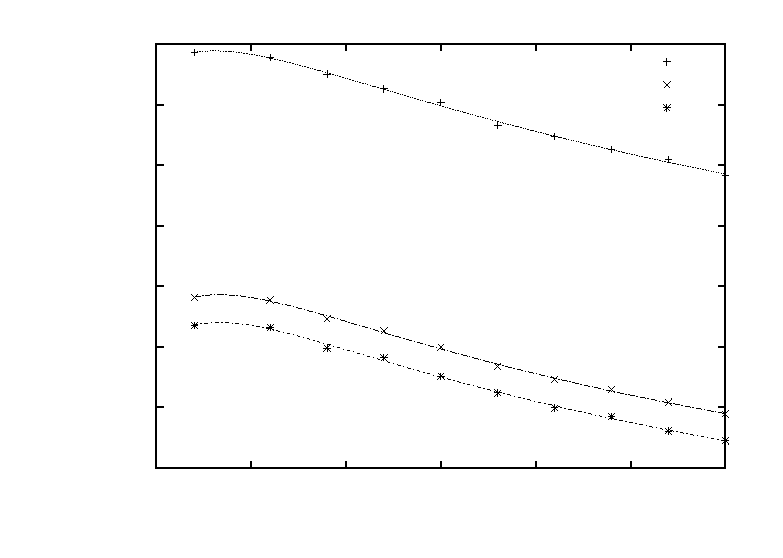
\includegraphics{GT}}%
    \gplfronttext
  \end{picture}%
\endgroup

\caption{Teplotní závislost indexu lomu vzorku 1.}
\label{GT}
\end{figure}


\subsection{Chyby}
Dle teoretického výpočtu ze vzorců \ref{N1} a \ref{N2} mi nepříma chyba výpočtu, za předpokladu, že $N_1$ mělo přesnost na poslední uvedenou cifru, zaokrouhleno na jednu platnou cifru 0.001 \% resp. 0.002 \%. Pro závislost na vlnové délce však získáme hodnotu o něco horší, protože určení její hodnoty je zatíženo relativně velkoou chybou.

\section{Diskuze}
Celé měření je zatíženo velmi malou chybou. To především díky přesnosti konstant použitých při výpočtech a samotnou přesností Pulfrichova refraktometru, který měří 
s přesností na desetinu minuty. Výsledné závislosti vyšli v oblasti vyšších vlnových délek velmi dobře. Pro nižší hodnoty se projevil nedostatek měřených hodnot, 
který byl způsoben chybějící vodíkovou trubicí, která by přidala dvě podstatné hodnoty. Celé spektrum rtuťové výbojky jsem také mohl přesněji proměřit bez filtru, 
čímž bych získal hodnoty z červené oblasti. U vzorku 9 jsem totiž naměřil "zelené" čáry, avšak jsem zapoměl na použitý filtr a tak nejsem sto stanovit, o které čáry se jednalo.
U kapaliny jsem zvolil metodu rychlého přechodu mezi teplotami a následné ponechání jemného topení na udržení teploty. Měření tak probíhalo vcelku rychle a v průběhu 
odečítání byla tepota vzorku v rozmezí čtvrt stupně celsia.

\section{Závěr}
Vynesl jsem disperzní křivku pro hranol GoF3, která je na obrázku \ref{GGoF3}. \\
Proměřil jsem závislost indexu lomu vzorků na vlnové délce. Hodnoty jsou v tabulkách \ref{T3}, \ref{T9} a závislosti na obrázcích \ref{G3}, \ref{G9}.\\
Určil jsem střední a relativní disperzi vzorků. Výsledky jsou v tabulce \ref{TDis}. Vypočetl jsem Abbeovo číslo.\\
Určil jsem, že se jedná o vzorky BK 7 a F2. \\
Proměřil jsem teplotní závislost indexu lomu vzorku jedna. \\
Z naměřených hodnot jsem stanovil, že se jednalo o ethanol.


\begin{thebibliography}{5}
	\bibitem{text} \textbf{Studijní text na praktikum III} \\http://physics.mff.cuni.cz/vyuka/zfp/txt\_310.htm (6. 4. 2012)
	\bibitem{text2} \textbf{Studijní text na praktikum III} \\http://physics.mff.cuni.cz/vyuka/zfp/txt\_309.htm (23. 3. 2012)
	\bibitem{text3} \textbf{Studijní text na praktikum III} \\http://physics.mff.cuni.cz/vyuka/zfp/txt\_303.htm (10. 2. 2012)
    \bibitem{chyba} \emph{J. Englich}: \textbf{Zpracování výsldků fyzikálních měření} \\ LS 1999/2000
    \bibitem{maly} \emph{prof. RNDr. Petr Malý , DrSc.}: \textbf{Optika}\\Univerzita Karlova v Praze, Nakladatelství Karolinum 2008, první vydání
\end{thebibliography}




\end{document}
